\subsection{Hauptoberfläche}

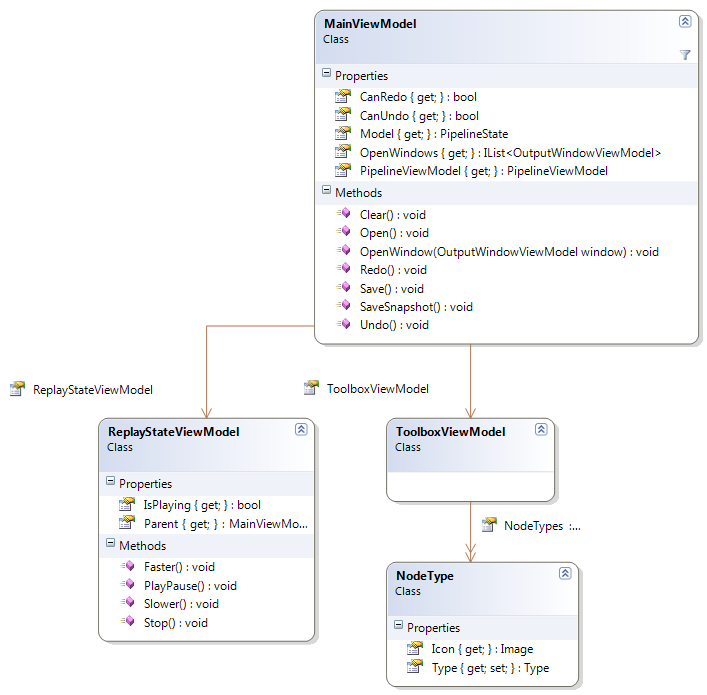
\includegraphics[width=\textwidth]{YuvKA.ViewModel/main.png}
Das Programm wird durch Instanzierung des \name{MainViewModel}s und Anzeigen der zugehörigen View gestartet. Diese Klasse delegiert Einheiten der Hauptoberfläche an untergeordnete View Models, wobei die Klassen zur Anzeige des Pipeline-Graphen erst im nächsten Abschnitt beschrieben werden.

\subsubsection{MainViewModel}

\begin{verbatim}
public class MainViewModel
\end{verbatim}

\paragraph{Beschreibung}~\\
Die \name{MainViewModel}-Klasse hält das Programm-Model in Form einer \name{PipelineState}-Instanz, verwaltet es in einem Undo/Redo-System und instanziert weitere untergeordnete View Models.

\paragraph{Typmember}
\begin{itemize}

\property{CanUndo, CanRedo}
	\begin{verbatim}
	public bool CanUndo { get; }
	public bool CanRedo { get; }
	\end{verbatim}
	Ruft ab, ob ein Rückgängig- bzw. Wiederholen-Schritt zur Verfügung steht.

\property{Model}
	\INPC
	\begin{verbatim}
	public PipelineState Model { get; }
	\end{verbatim}
	Stellt das derzeitige Model-Objekt für Data Binding und untergeordnete View Models zur Verfügung.

\property{OpenWindows}
	\begin{verbatim}
	public IList<OutputWindowViewModel> OpenWindows { get; }
	\end{verbatim}
	Ruft eine Liste der derzeit geöffneten Ausgabefenster ab.

\property{ReplayStateViewModel, PipelineViewModel, ToolboxViewModel}
	Ruft jeweils eine Instanz der gleichnamigen Klasse ab.

\method{Clear, Open}
	\begin{verbatim}
	public void Clear()
	public void Open()
	\end{verbatim}
	Ersetzen das derzeitige Model durch eine neue leere bzw. aus einer Datei geladenen Pipeline, dabei wird jeweils ein neuer Rückgangig-Schritt erzeugt. Open öffnet zusätzlich einen \name{OpenFileDialog} zur Auswahl des Dateipfades.

\method{Save}
	\begin{verbatim}
	public void Save()
	\end{verbatim}
	Speichert das derzeitige Model in einer Datei ab. Dazu öffnet Save einen \name{SaveFileDialog} und serialisiert dann das \name{Model}-Objekt in die gewählte Datei.

\method{SaveSnapshot()}
	\begin{verbatim}
	public void SaveSnapshot()
	\end{verbatim}
	Hält den aktuellen Model-Zustand als Rückgängig-Schritt fest. Alle Wiederholen-Schritte werden verworfen.

\method{Undo, Redo}
	\begin{verbatim}
	public void Undo()
	public void Redo()
	\end{verbatim}
	Stellt den Zustand des nächsten Rückgängig- bzw. Wiederholen-Schrittes wieder her.

\end{itemize}